% -*- TeX:Rnw -*-
% ----------------------------------------------------------------
% .R Sweave file  ************************************************
% ----------------------------------------------------------------
%%
% \VignetteIndexEntry{}
% \VignetteDepends{}
% \VignettePackage{}
%\documentclass[a4paper,12pt]{article}
\usepackage[slovene]{babel}
\usepackage[cp1250]{inputenc} %% must be here for Sweave encoding check
\newcommand{\SVNRevision}{$ $Rev: 3 $ $}
%\newcommand{\SVNDate}{$ $Date:: 2009-02-2#$ $}
\newcommand{\SVNId}{$ $Id: program.Rnw 3 2009-02-22 17:36:08Z ABlejec $ $}
%\usepackage{babel}
%\input{abpkgB}
%\input{abpkg}
\input{abBeam}
\input{abcmd}
%\input{abpage}
\usepackage{pgf,pgfarrows,pgfnodes,pgfautomata,pgfheaps,pgfshade}
\usepackage{amsmath,amssymb}
\usepackage{colortbl}
\usepackage{Sweave}
\input{mysweaveB}
\newcommand{\BV}{}
\newcommand{\EV}{}
\newcommand{\myemph}[1]{{\color{Sgreen} \textit{#1}}}
\input{./figs/Verjetnost-concordance}
%\SweaveOpts{echo=false}
%\usepackage{lmodern}
%\input{abfont}

% ----------------------------------------------------------------
\title{Iskanje biserov:\\Verjetnostne funkcije}
\author{A. Blejec}
%\address{}%
%\email{}%
%
%\thanks{}%
%\subjclass{}%
%\keywords{}%

%\date{}%
%\dedicatory{}%
%\commby{}%
\begin{document}
\mode<article> {\maketitle}
\mode<presentation> {\frame{\titlepage}}
\tableofcontents
% ----------------------------------------------------------------
\begin{abstract}
 
\end{abstract}
% -------------------------------------------------------------
%% Sweave settings for includegraphics default plot size (Sweave default is 0.8)
%% notice this must be after begin{document}
% \setkeys{Gin}{width=0.9\textwidth}
\setkeys{Gin}{width=0.7\textwidth}
% ----------------------------------------------------------------
%% |--------------------->>>>>>
\begin{frame}[fragile]
\frametitle{Tabla pred nekaj tedni ...}
\begin{center}
  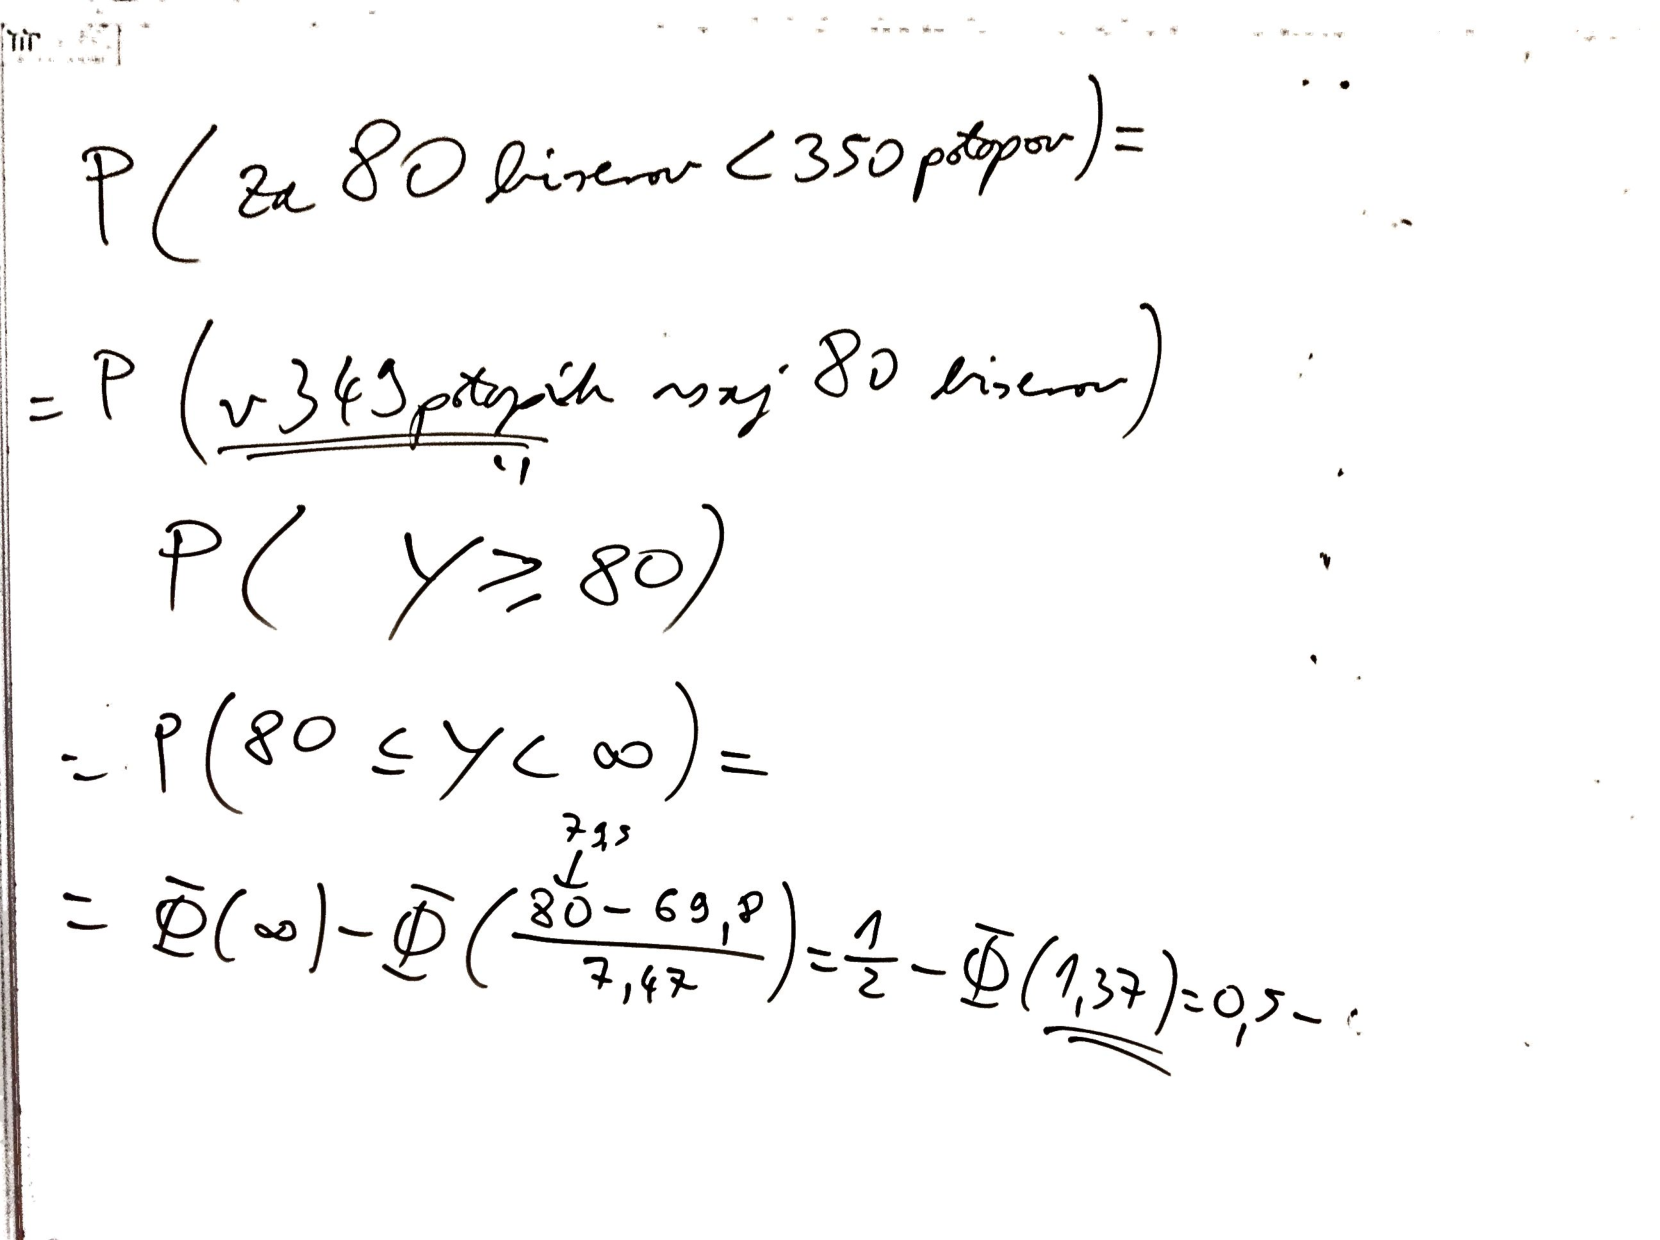
\includegraphics[width=\textwidth]{../clp/Verjetnost1.pdf}
\end{center}
\end{frame}
%% <<<<<<---------------------|

%% |--------------------->>>>>>
\begin{frame}[fragile]
\frametitle{Tabla pred nekaj tedni ...}
\begin{center}
  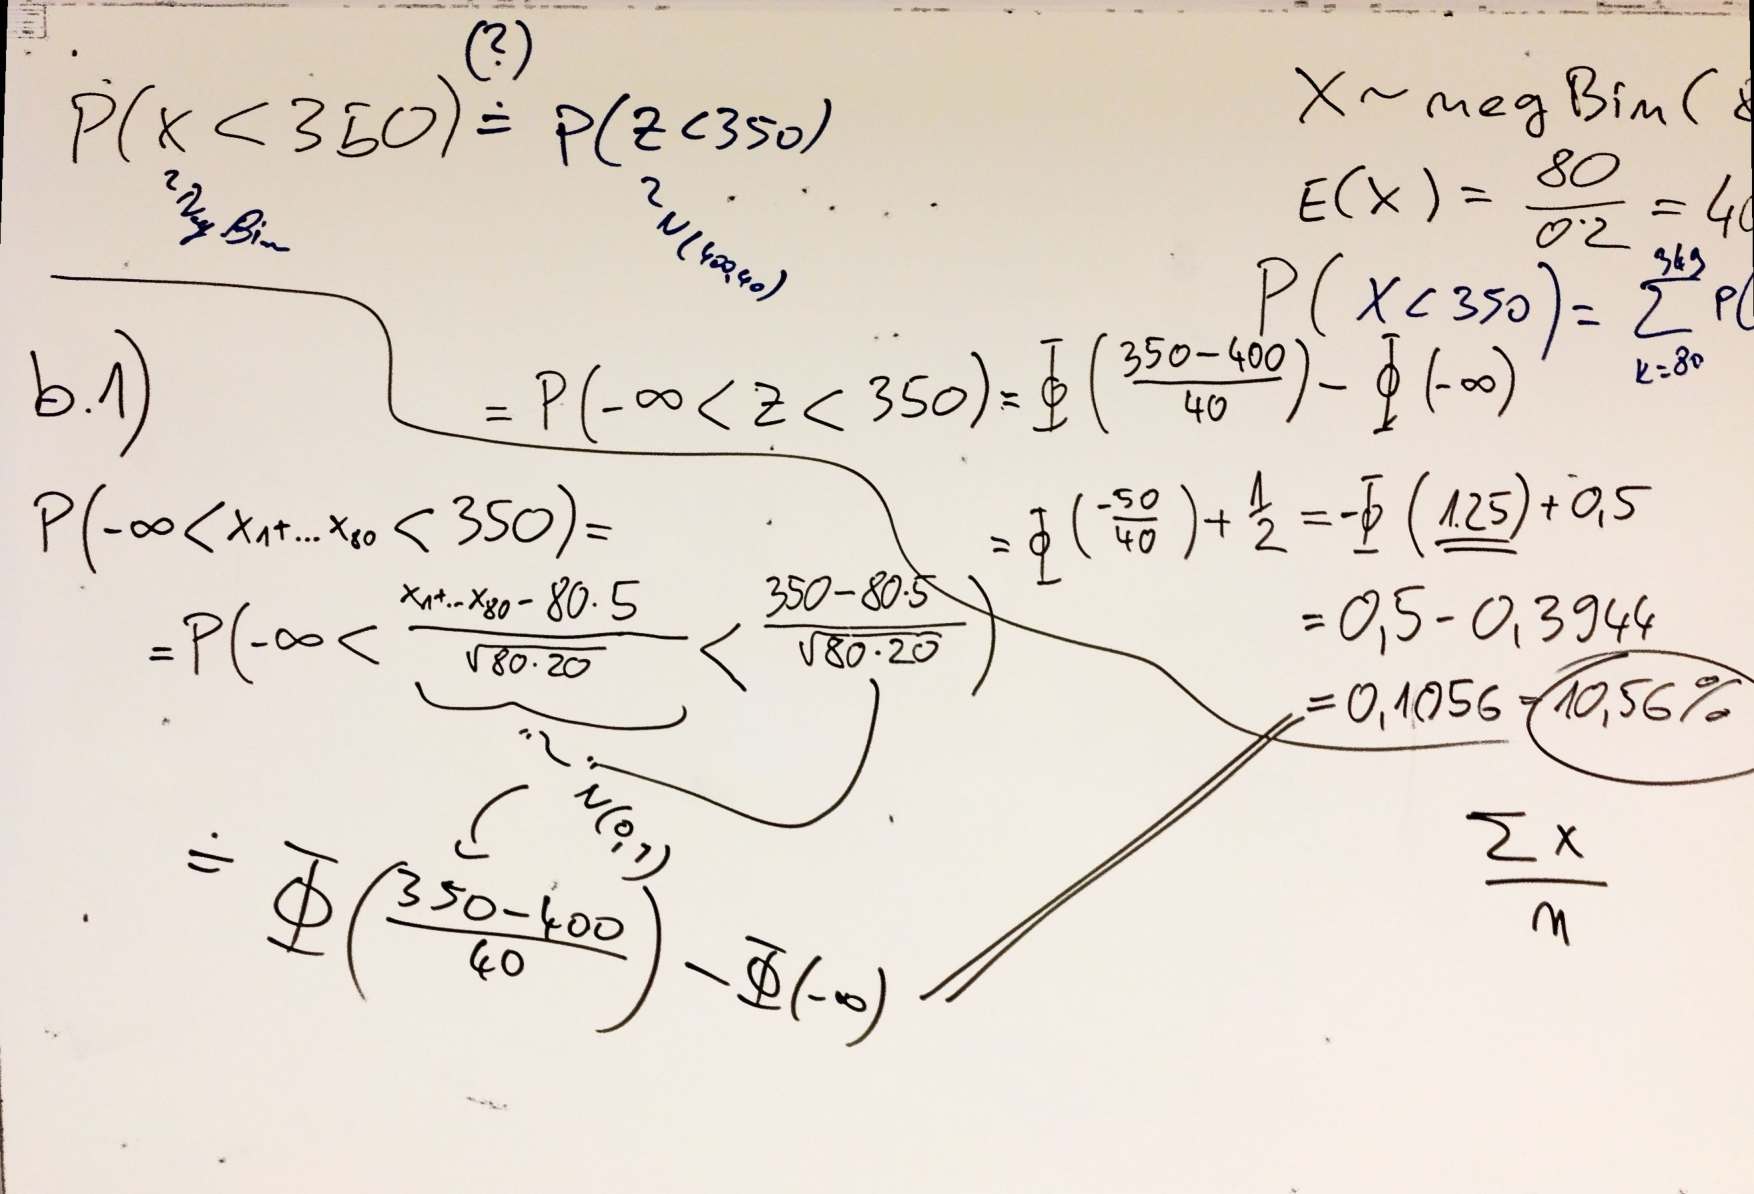
\includegraphics[width=\textwidth]{../clp/Verjetnost3.pdf}
\end{center}
\end{frame}
%% <<<<<<---------------------|

%% |--------------------->>>>>>
\begin{frame}[fragile]
\frametitle{Tabla pred nekaj tedni ...}
\begin{center}
  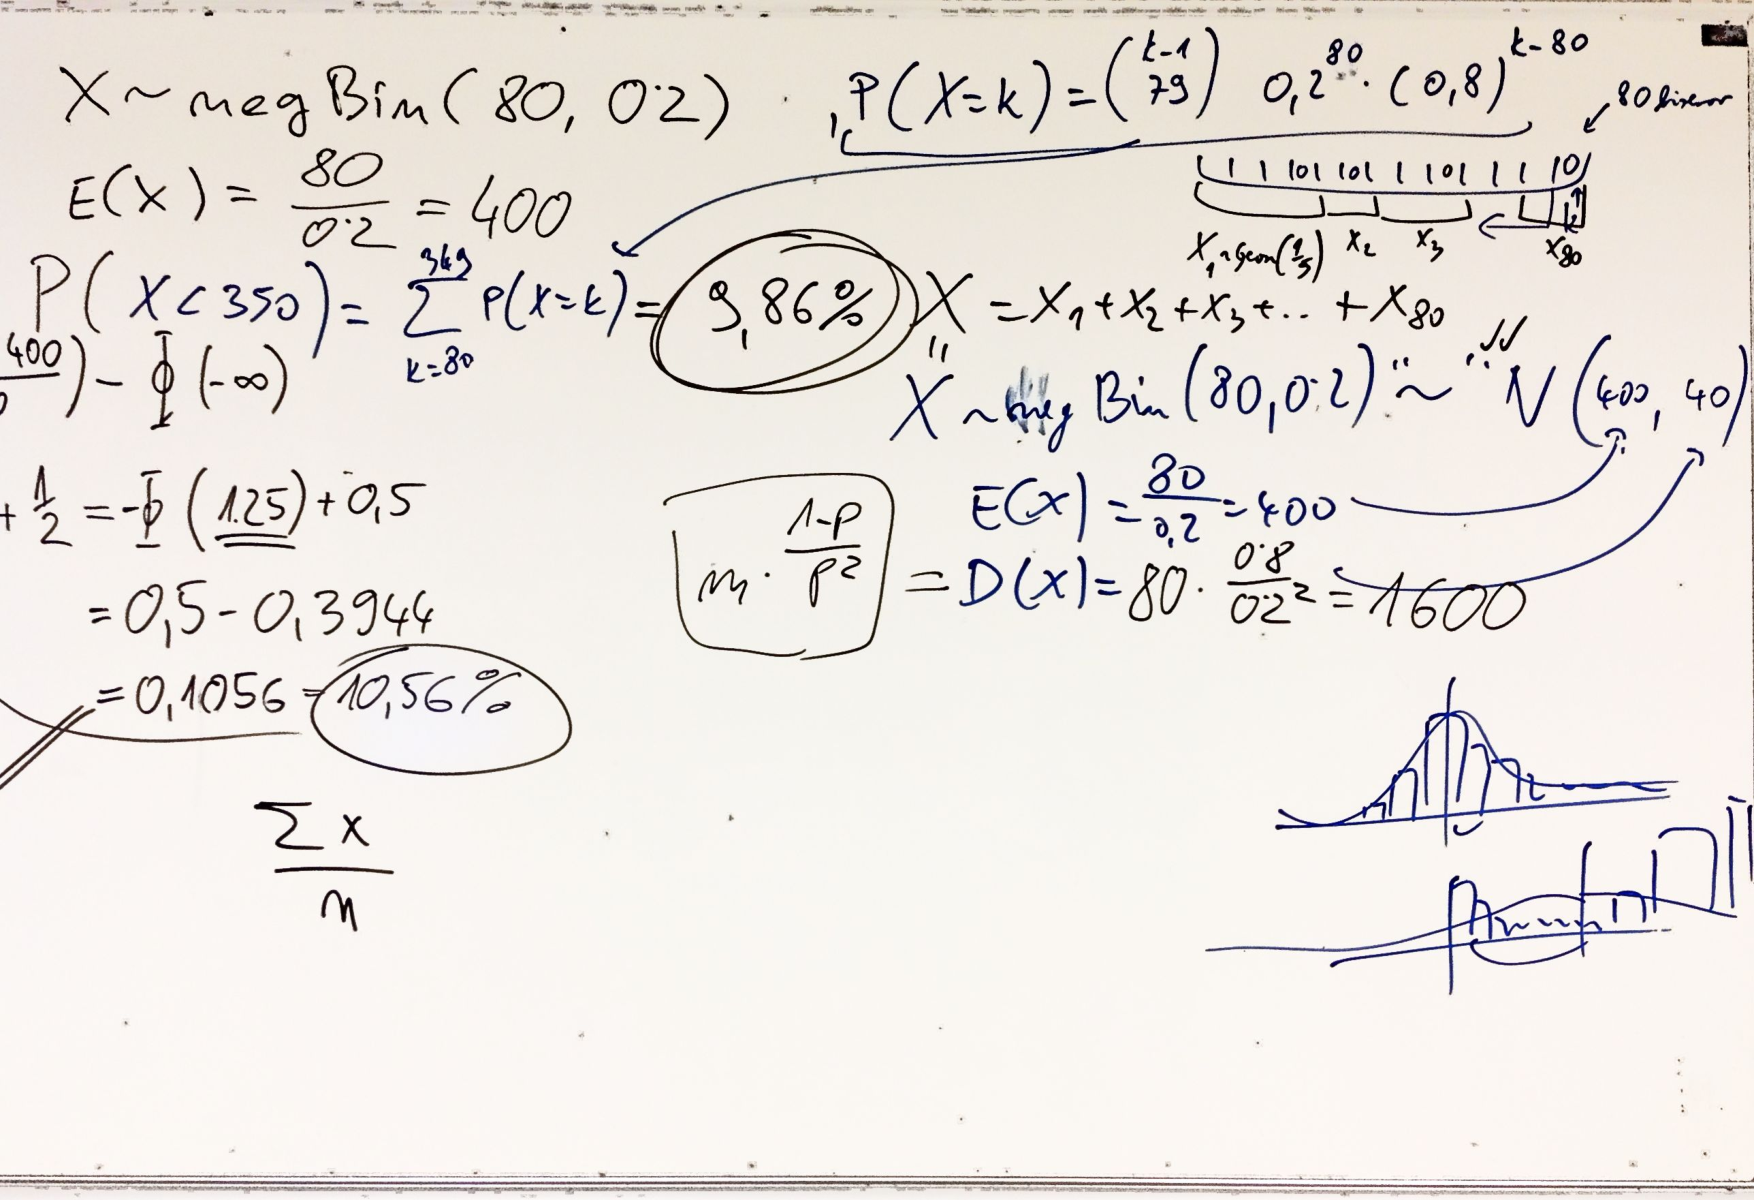
\includegraphics[width=\textwidth]{../clp/Verjetnost2.pdf}
\end{center}
\end{frame}
%% <<<<<<---------------------|



%% |--------------------->>>>>>
\begin{frame}[fragile]
\frametitle{Negativna binomska porazdelitev}
$$X \sim negBin(n=80,p=0.2)$$
$$P(X = k) = {k-1 \choose n-1} p^n \cdot(1-p)^{k-n}$$

\begin{Schunk}
\begin{Sinput}
> n <- 80
> k <- 350
> p <- 0.2
> choose(k - 1, n - 1) * p^n * (1 - p)^(k - n)
\end{Sinput}
\begin{Soutput}
[1] 0.004890492
\end{Soutput}
\end{Schunk}
V R je funkcija parametrizirana na �tevilo neuspehov.
\begin{Schunk}
\begin{Sinput}
> dnbinom(k - n, n, p)
\end{Sinput}
\begin{Soutput}
[1] 0.004890492
\end{Soutput}
\begin{Sinput}
> pnbinom(k - n, n, p) - pnbinom(k - n - 1, n, p)
\end{Sinput}
\begin{Soutput}
[1] 0.004890492
\end{Soutput}
\end{Schunk}
$$P(X \leq 350)$$
\begin{Schunk}
\begin{Sinput}
> pnbinom(k - n, n, p)
\end{Sinput}
\begin{Soutput}
[1] 0.1034488
\end{Soutput}
\end{Schunk}
\end{frame}
%% <<<<<<---------------------|


%% |--------------------->>>>>>
\begin{frame}[fragile]
\frametitle{Normalna aproksimacija}
$$X \sim negBin(n=80,p=0.2)$$
$$E(X)=\frac{n}{p}=\frac{80}{0.2}=400$$
$$D(X)=\frac{80*0.8}{0.2^2}=1600$$
$$X \sim N(400,40^2)$$
$$P(X \leq 350)$$
\begin{Schunk}
\begin{Sinput}
> pnorm(350, 400, 40)
\end{Sinput}
\begin{Soutput}
[1] 0.1056498
\end{Soutput}
\end{Schunk}
\end{frame}
%% <<<<<<---------------------|

%% |--------------------->>>>>>
\begin{frame}[fragile]

\frametitle{Geometrijska porazdeitev}
\begin{Schunk}
\begin{Sinput}
> n <- 80
\end{Sinput}
\end{Schunk}
$$X_k \sim geom(p=0.2),\  k= 1, 2, \ldots, 80$$
Koliko poskusov do prvega uspeha
$$P(X = k)=(1-p)^{k-1}*p, k=1, 2, \ldots$$
\vspace{-1cm}
\begin{Schunk}
\begin{Sinput}
> set.seed(789)
> X <- rgeom(n, p = 0.2) + 1
> X[1:5]
\end{Sinput}
\begin{Soutput}
[1]  1 20 16  5  5
\end{Soutput}
\begin{Sinput}
> (Y <- sum(X))
\end{Sinput}
\begin{Soutput}
[1] 454
\end{Soutput}
\end{Schunk}
Zakaj $+1$ ? Poglejte v pomo� funkcije \code{rgeom}.
\end{frame}
%% <<<<<<---------------------|

%% |--------------------->>>>>>
\begin{frame}[fragile]
\frametitle{Potaplja�ki poskus}
\vspace{-0.5cm}
\begin{Schunk}
\begin{Sinput}
> par(mar = c(3, 3, 2, 1), mgp = c(2, 0.7, 0))
> X <- c(0, X)
> plot(cumsum(X), 0:n, type = "s", ylab = "Biserov", 
+     xlab = "�tevilo potopov")
> points(cumsum(X[-1]), 1:n, col = "red", pch = 16, 
+     cex = 0.5)
\end{Sinput}
\end{Schunk}
\includegraphics{./figs/Verjetnost-009}
\end{frame}
%% <<<<<<---------------------|

%% |--------------------->>>>>>
\begin{frame}[fragile]
\frametitle{Simulacija}
\begin{Schunk}
\begin{Sinput}
> n <- 350
> skoljka <- c("prazna", "biser")
> izid <- sample(skoljka, n, replace = TRUE)
> table(izid)
\end{Sinput}
\begin{Soutput}
izid
 biser prazna 
   177    173 
\end{Soutput}
\end{Schunk}
\end{frame}
%% <<<<<<---------------------|

%% |--------------------->>>>>>
\begin{frame}[fragile]
\frametitle{Simulacija z neenako verjetnostjo}
\begin{Schunk}
\begin{Sinput}
> n <- 350
> skoljka <- c("prazna", "biser")
> izid <- sample(skoljka, n, replace = TRUE, prob = c(8, 
+     2))
> (t <- table(izid))
\end{Sinput}
\begin{Soutput}
izid
 biser prazna 
    83    267 
\end{Soutput}
\begin{Sinput}
> t["biser"]/sum(t)
\end{Sinput}
\begin{Soutput}
    biser 
0.2371429 
\end{Soutput}
\end{Schunk}
\end{frame}
%% <<<<<<---------------------|

%% |--------------------->>>>>>
\begin{frame}[fragile]
\frametitle{Drug pristop}

\begin{Schunk}
\begin{Sinput}
> p0 <- 0.2
> izid <- runif(n) <= p0
> (t <- table(izid))
\end{Sinput}
\begin{Soutput}
izid
FALSE  TRUE 
  296    54 
\end{Soutput}
\begin{Sinput}
> t[2]/sum(t)
\end{Sinput}
\begin{Soutput}
     TRUE 
0.1542857 
\end{Soutput}
\end{Schunk}
Z logi�nimi vrednostmi lahko ra�unamo:
\begin{Schunk}
\begin{Sinput}
> sum(izid)
\end{Sinput}
\begin{Soutput}
[1] 54
\end{Soutput}
\begin{Sinput}
> sum(izid)/length(izid)
\end{Sinput}
\begin{Soutput}
[1] 0.1542857
\end{Soutput}
\end{Schunk}

\end{frame}
%% <<<<<<---------------------|

%% |--------------------->>>>>>
\begin{frame}[fragile]
\frametitle{Veliko �tevilo potaplja�ev N}
\begin{Schunk}
\begin{Sinput}
> N <- 100
> n <- 350
> p <- 0.2
> X <- matrix(runif(N * n) <= p, N, n)
> X[1:4, 1:10] + 0
\end{Sinput}
\begin{Soutput}
     [,1] [,2] [,3] [,4] [,5] [,6] [,7] [,8] [,9] [,10]
[1,]    1    0    0    0    0    0    0    0    0     0
[2,]    0    1    0    0    0    0    0    1    1     0
[3,]    1    1    0    1    0    0    0    0    0     0
[4,]    0    0    1    0    0    0    1    0    0     0
\end{Soutput}
\end{Schunk}
\begin{Schunk}
\begin{Sinput}
> biserov <- apply(X, 1, sum)
> head(biserov)
\end{Sinput}
\begin{Soutput}
[1] 66 57 56 76 65 66
\end{Soutput}
\end{Schunk}
\end{frame}
%% <<<<<<---------------------|

%% |--------------------->>>>>>
\begin{frame}[fragile]
\frametitle{Porazdelitev}
\begin{Schunk}
\begin{Sinput}
> hist(biserov, col = "lightblue")
\end{Sinput}
\end{Schunk}
\includegraphics{./figs/Verjetnost-016}
\end{frame}
%% <<<<<<---------------------|

%% |--------------------->>>>>>
\begin{frame}[fragile]
\frametitle{�tevilo potopov za 80 biserov}
Z vsoto geometrijskih ali pa z negativno binomsko porazdelitvijo
\begin{Schunk}
\begin{Sinput}
> N <- 10000
> n <- 80
> p <- 0.2
> X <- matrix(rgeom(N * n, p = p), N, n) + 1
> X[1:4, 1:10]
\end{Sinput}
\begin{Soutput}
     [,1] [,2] [,3] [,4] [,5] [,6] [,7] [,8] [,9] [,10]
[1,]    9    3    6    8    3    2   10    4    4     3
[2,]    3    3   10    2    7    9    1    4    1     1
[3,]    3    7    8    1    1    4    1    4    7    18
[4,]    2    1    2    2    3    7    2    7    4     1
\end{Soutput}
\end{Schunk}

\begin{Schunk}
\begin{Sinput}
> potopov <- apply(X, 1, sum)
> head(potopov)
\end{Sinput}
\begin{Soutput}
[1] 422 367 408 369 393 350
\end{Soutput}
\end{Schunk}

\end{frame}
%% <<<<<<---------------------|

%% |--------------------->>>>>>
\begin{frame}[fragile]
\frametitle{Porazdelitev �tevila potopov}
\begin{Schunk}
\begin{Sinput}
> p <- sum(potopov <= 350)/length(potopov)
> hist(potopov, col = "lightblue", main = p)
> abline(v = 350, col = "red")
\end{Sinput}
\end{Schunk}
\includegraphics{./figs/Verjetnost-019}
\end{frame}
%% <<<<<<---------------------|

%%% |--------------------->>>>>>
%\begin{frame}[fragile]
%\frametitle{Simulacija z negativno binomsko porazdelitvijo}
%<<>>=
%N <- 10000
%n <- 80
%p <- 0.2
%potopov <- rnbinom(N,n,p)
%head(potopov)
%hist(potopov,col="lightblue",main=sum(potopov<=350)/length(potopov))
%
%@
%\end{frame}
%%% <<<<<<---------------------|





% ----------------------------------------------------------------
\bibliographystyle{amsplain}
\bibliography{ab-general}
\end{document}
% ----------------------------------------------------------------
